\section{Theorie}
\label{sec:Theorie}

\subsection{Grundlagen Laser Physik}
Das englische Synonym Laser steht für \textit{light amplification by stimulated emission of radiation}
und bezeichnet den physikalischen Effekt mit dem  Laserstrahlen erzeugt werden.
Im Unterschied zu anderen Lichtquellen emittieren Laser Licht der Gleichen Wellenlänge, Phase ,Polarisation und Richtung. 
Daher Stellen sie in der Experimentalphysik ein Wichtiges Instrument dar,
zum Beispiel bei der Untersuchung von Materialien.

Ein Laser besteht Typischerweise aus drei Bauteilen. Das \textit{aktive Medium}, die \textit{Pumpe} und den \textit{Resonator}.
Im aktiven Medium werden durch Quantensprünge von Elektronen auf niedrigere Energie Niveaus Photonen emittiert.
Diese Abfallen auf niedrigere Niveaus kann verschieden ablaufen (vgl. \ref{fig:emmision}).
\begin{figure}[h]
    \centering
    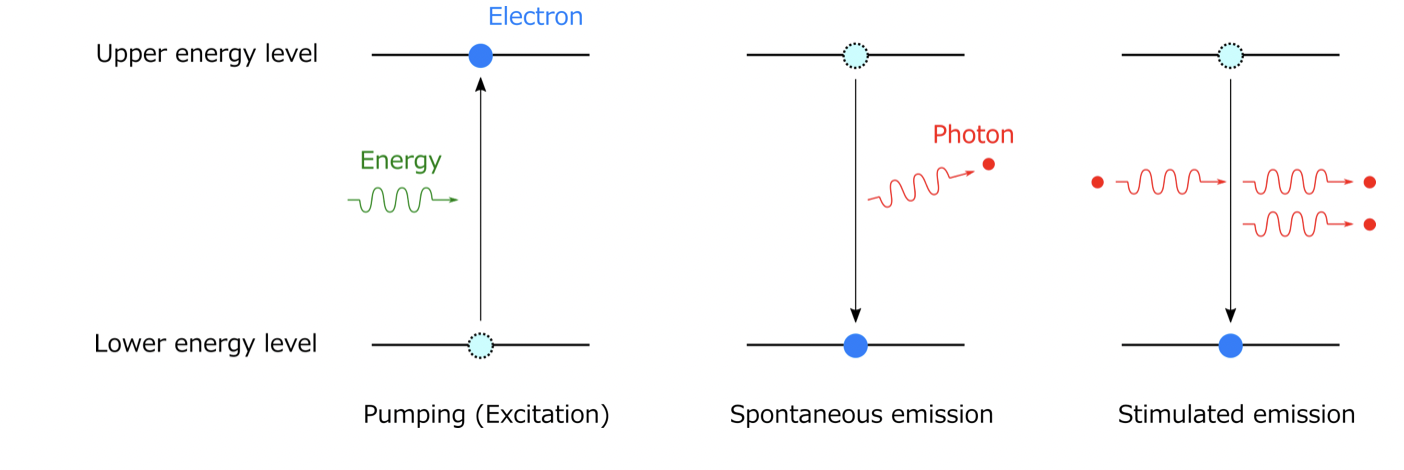
\includegraphics[width=0.7\textwidth]{abb/emission.png}
    \caption{Absorption spontane Emission und stimulierte Emission \cite{emission}}
    \label{fig:emmision}
\end{figure}
Um monochromatische, kohärente Strahlung zu emittieren ist besonders die stimulierte Emission von Bedeutung,
da bei der spontanen Emission Richtung und Phase des emittierten Photons zufällig auftreten.
Bei der stimulierten Emission hingegen fällt das Elektron erst durch die Stimulation eines Photons auf das niedrigere Energieniveau,
dabei wird ein Photon mit exakt den selben Eigenschaften wie die des Stimulierende Photon erzeugt.
Das so entstandene zweite Atom kann nun selber andere Elektronen stimulieren,
so dass es zu einer Kettenreaktion kommt. 
Durch den Resonator, 
Welcher meist aus zwei Spiegeln besteht,
die mit passendem Abstand zur Wellenlänge positioniert sind,
durchlaufen die Photonen das Lasermedium mehrmals,
was die Chance, ein weiteres Elektron zu stimulieren, erhöht. 
Einer der beiden Spiegel ist Lichtdurchlässig, wodurch die Photonen zur Nutzung austreten können.
Um das Prinzip der stimulierten Emission nutzen zu können,
muss im aktiven Medium ein Zustand der Besetzungsinversion hergestellt werden.
Also, 
dass der energiereichere Zustand mit höherer Wahrscheinlichkeit besetzt ist als der Energie niedrigere.
In einem zwei Zustand System kann eine solche Besetzungsinversion nicht hergestellt werden,
da sich Absorption und stimulierte Emission gerade ausgleichen.  
Erst mit einem dritten Energieniveau (vgl. \refeq{fig:dreiniveau}) ist eine Besetzungsinversion möglich.
\begin{figure}[h]
    \centering
    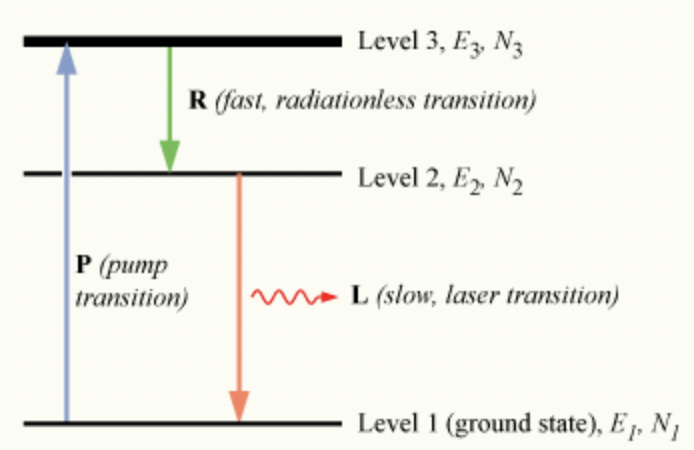
\includegraphics[width=0.5\textwidth]{abb/dreiniveau.png}
    \caption{Besetzungsinversion im drei-Zustandssystem \cite{enwiki}}
    \label{fig:dreiniveau}
\end{figure}
Die Elektronen werden vom System von Niveau 1 auf Niveau 3 gepumpt. 
Dort gehen sie weitgehend strahlungsfrei in Niveau 2 über, 
um dann durch stimulierte Emission wieder in Niveau 1 zu fallen.
Da der Pump Vorgang nicht das mittlere Niveau anspricht,
kann dort eine höhere Besetzungszahl erzeugt werden. 
